\documentclass{article}
\usepackage{listings}
\usepackage{mathrsfs}
\usepackage[utf8]{inputenc}
\usepackage{amssymb}
\usepackage{lipsum}
\usepackage{amsmath}
\usepackage{fancyhdr}
\usepackage{geometry}
\usepackage{scrextend}
\usepackage[english,german]{babel}
\usepackage{titling}
\setlength{\droptitle}{-3cm}
\usepackage{tikz}
\usepackage{algorithm,algpseudocode}
\usepackage[doublespacing]{setspace}
\usetikzlibrary{datavisualization}
\usetikzlibrary{datavisualization.formats.functions}
\usepackage{polynom}
\usepackage{amsmath}
\usepackage{gauss}
\usepackage{tkz-euclide}
\usepackage{minted}
\usepackage{mathrsfs}
\usetikzlibrary{datavisualization}
\usetikzlibrary{datavisualization.formats.functions}
\author{
Alexander Mattick Kennung: qi69dube\\
Kapitel 1
}
\usepackage{import}
\date{\today}
\geometry{a4paper, margin=2cm}
\usepackage{stackengine}
\parskip 1em
\newcommand\stackequal[2]{%
  \mathrel{\stackunder[2pt]{\stackon[4pt]{=}{$\scriptscriptstyle#1$}}{%
  $\scriptscriptstyle#2$}}
 }
\makeatletter
\renewcommand*\env@matrix[1][*\c@MaxMatrixCols c]{%
  \hskip -\arraycolsep
  \let\@ifnextchar\new@ifnextchar
  \array{#1}}
\makeatother
\lstset{
  language=haskell,
}
\lstnewenvironment{code}{\lstset{language=Haskell,basicstyle=\small}}{}
\usepackage{enumitem}
\setlist{nosep}
\usepackage{titlesec}
\usepackage{ stmaryrd }
\usepackage{verbatim}
\usepackage{tikz-qtree}
\usepackage{bussproofs}

\titlespacing*{\subsection}{0pt}{2pt}{3pt}
\titlespacing*{\section}{0pt}{0pt}{5pt}
\titlespacing*{\subsubsection}{0pt}{1pt}{2pt}
\title{Übung 7}


\begin{document}
	Thema: Abstiegsverfahren\\
  Gegeben: Quadratisches Funktional.\\
  \[Q(\vec{x}) = x^TAx +2b^Tx+c\]
  $A\in\mathbb{R}^{n\times n}$ ist symmetrisch positiv definit.\\
  $b\in\mathbb{R}^n$\\
  gesucht.: minimalstelle\\
  Methode gradient descent:\\
  \[x_{i+1} =  x_i - t_i\cdot \nabla f(x_i)\]
  optimale schrittweite $\tau$, sodass
  $x_1 = x_0 +\tau\cdot s_0$\\
  suche $\tau$, sodass $Q(x_1)$ minimal wird.\\
  wir haben also ein eindimensionales optimierungsproblem in $\tau$.
  \[q(\tau) = Q(x_0+\tau\cdot s_0)\]
  wir wissen, dass $q(\tau)$ eine 1-d parabel entlang des gradienten auf der quadratischen Funktion ist\\
  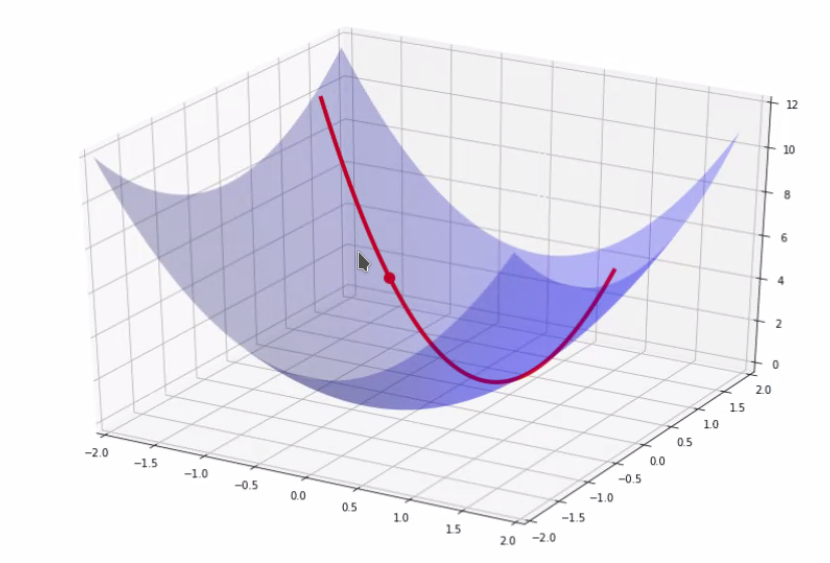
\includegraphics{tau.png}\\
  \[q(\tau)d/d\tau = d/d\tau Q(x_0+\tau\cdot s_0)\]
  Kettenregel
  \[q(\tau)d/d\tau = dQ/dx\ Q(x_0+\tau\cdot s_0) \cdot d/d\tau\ (x_0+\taus_0)\]
  \[(\nabla Q(x_0+\taus_0))^T\cdot s_0\]
  \[<\nabla Q(x_0+\taus_0)), s_0>\]
  der Gradient steht senkrecht auf der Suchrichtung: der Erste komponent ist präzise das, was wir optimieren wollen!\\
  \[\nabla Q(x) = 2Ax+2b\]
  also folgt für $\tau$
  \[<2(A(x_0+\tau s_0)+b), s_0>\]
  \[<2(Ax_0+A\tau s_0+b), s_0>\]
  \[2((Ax_0)^T s_0 + \tau(As_0)^T s_0 +b^T s_0)=0\]
  \[\iff \tau (As_0)^Ts_0 = -((Ax_0)^T s_0+b^T s_0)\]
  \[\iff \tau  = -\frac{<Ax_0+b,s_0>}{<As_0,s_0>}\]
  Für Tau betrachten wir also das  verhältniss vom inneren produkt der suchrichtung zur 1. ableitung des momentanen punktes und der Suchrichtung und 2. ableitung.\\
  gradientenverfahren: Suchrichtung ist Gradient.\\
  A konjugation:\\
  bisher: gehen vom gradienten im schnellsten weg zur nächsten niveaulinie. $<s_1,s_0>=0$ für den nächsten wert.\\
  A konjugation ändert das krit. auf $<s_1,As_0>=0$ \\
  für uns hier $s_1^T (-4,-8)^T=0\implies s_1= (2,-1)^T$\\
  f)\\
  1. Schritt gleich gradientenverfahren:\\
  $x_1 = x_0+\tau_0 s_0 = (-1,1)^T$\\
  2. Schritt\\
  wir gehen in richtung des konj. Gradienten. (also hier das zuvor berechnete $s_1$)\\
  $\tau_1 = \frac{<Ax_1+b,s_1>}{>As_1,s_1>} = 1/7$\\
  $y_2 = (-5/7, 6/7)^T$\\
  WIR SIND AM NULLPUNKT (weil wir exakt rechnen und quadratisch sind)\\
  Reading zu CG:\\
  ``conjugate gradients without the agonizing pain''\\


\end{document}
